\documentclass[a4paper,12pt,oneside, bibliography=totoc]
{scrbook}
\usepackage[utf8]{inputenc}

% Schrift und -kodierung
\usepackage[T1]{fontenc}
\usepackage{lmodern}

% Sprache/Silbentrennung
\usepackage[german]{babel} %TODO change to german if desired
\usepackage{booktabs}
\usepackage{amsmath}
\usepackage{floatflt}
\usepackage{float} 
\usepackage{graphicx}
\usepackage{pbox}
\usepackage{algorithmic}
\usepackage{algorithm}
\usepackage{siunitx}
\usepackage[autostyle]{csquotes}
\usepackage{todonotes}

\usepackage[page, title, titletoc, header]{appendix} %prettier appendix



\usepackage[printonlyused]{acronym}
\usepackage{listings} 
\usepackage{subfig}
\lstset{xleftmargin=2em} %Proper indention of listings


\usepackage{tabularx} %For tables
\usepackage{csquotes} %For Quotes





%Footnote Numbering not reset in new chapters
\usepackage{chngcntr}
\counterwithout{footnote}{chapter}


%Remove last point after section/subsections
\renewcommand{\autodot}{}

\usepackage[htt]{hyphenat} %damit texttt noch Linebreaks mit Silbentrennung erzeugt
\newcommand{\code}[1]{\texttt{#1}} %Programmcode im Textfluss in passendem Font ausgeben




   
%Literatur
%Ordering in references checken, vermutlich was mit style=numeric zu tun
\usepackage[
   backend=biber,
   sorting= none,
   firstinits=true,
   date=long,
   urldate=long
]{biblatex}
\addbibresource{database.bib}
%\addbibresource{literatur2.bib}


\usepackage[]{hyperref}

\begin{document}
\frontmatter %roman page numbers





	\titlehead{
	\begin{center}
	   \includegraphics[width=10cm]{figures/unilogo.pdf}\\
	   	Institute of Computer Science, Software Engineering Group
	\end{center}
	}
	\subject{Bachelorarbeit, Masterarbeit}
	\title{Titel der Abschlussarbeit }
	\author{Vorname Nachname\\ Immatrikulationsnummer: 95XXXX} %engl. Matriculation Number

	\date{18.10.2018 \\
	Advisor: Prof. Dr.-Ing. Elke Pulvermüller \\ %Deutsch: Erstebetreuer
	Co-Advisor: Dennis Ziegenhagen, M.Sc.} %Deutsch: Zweitbetreuer
	
	\maketitle
	
	\clearpage
	
	\addchap*{Abstract}
\textbf{Deutsch}
Die Softwaredokumentation ist ein essentieller Bestandteil der heutigen Softwareentwicklung geworden. Nichtsdestotrotz leidet die Qualität der Dokumentation häufig und viele Entwickler sind nicht motiviert genug, um eine gute Dokumentation zu schreiben. Das Ziel dieser Arbeit ist es, ein Tool zu entwickeln, dass exemplarisch die Dokumentationsqualität von Javaprogrammen analysiert und mittels verschiedener Metriken bewertet. Dieses Tool soll anschließend in GitHub Actions eingebunden werden, um den Entwickler bei einer sehr schlechten Dokumentationsqualität zu warnen und gegebenenfalls Push- oder Mergevorgänge zu verhindern.

%\linebreak
\bigskip

\noindent
%\bigskip
\textbf{English} 
The software documentation has become an integral part of software development. Nevertheless, the quality of the documentation is often poor and developers are often not motivated to write good documentation. The goal of this thesis is to develop a tool that can analyze the quality of Java application by applying different metrics. This tool shall be integrated in Github Action to warn the developer about poor software documentation quality and to prevent a push or merge if the quality becomes too poor.  

%TODO Bis jetzt nur Osi Abstract, evtl. etwas ausführlicher für Masterarbeit


	\clearpage
	
	\tableofcontents
	\clearpage

	






\mainmatter %switch roman auf arabic page numbers
\chapter{Introduction}
\setcounter{page}{1} %Seitenzahlen hier mit 1 anfangen

	%Include text from other files into the document --> great for structuring
	\label{sec:introduction}

Ein wichtiger Bestandteil der Softwareentwicklung von heute ist die Softwaredokumentation. Dies liegt unter anderem daran, dass die Größe von Softwareprojekten steigt, so dass kein Entwickler das gesamte Programm im Überblick hat und daher zusätzliche Informationen neben dem Code benötigt [\ref{software_complexity}]. Nichtsdestotrotz wird die Softwaredokumentation von Entwicklern oft vernachlässigt [\ref{quality_analysis}].  Die Gründe für schlechte Dokumentation sind vielfältig. Das Schreiben der Dokumentation wird oft als mühevoll empfunden und erfordert Skills, die ein Programmierer nichts zwangsläufig hat[\ref{javadocMiner}] [\ref{comment_code}].  

Die mangelhafte Dokumentation führt dazu, dass nicht nur nachfolgende Entwickler Probleme mit dem Codeverständnis haben, sondern auch der Entwickler eines Moduls nach einer längeren Pause Zeit aufbringen muss, um den Code wieder zu verstehen. Auch für Kunden/Auftraggeber ist eine gute Dokumentation wichtig, da gut dokumentierte Software tendenziell besser wartbar ist und somit mehr Nutzen bringt [\ref{quality_analysis}][\ref{doc_managment_survey}].



\chapter{Problemstellung Softwaredokumentation}
	%Multiple input files for larger chapters are also possible
	\label{sec:background}
In diesen Kapitel soll die Problemstellung der mangelhaften Softwaredokumentation analysiert werden. Hierzu muss zunächst der Begriff \enquote{Softwaredokumentation} definiert werden. Anschließend werden einige Statistiken präsentiert, die zeigen, dass eine mangelhafte Softwaredokumentation ein reales Problem für Entwickler ist. Des Weiteren sollen die Folgen von schlecht dokumentierten Code analysiert werden. Zudem wird in diesem Kapitel die Grundlagen von Javadocs erläutert, welches das Tool später als Grundlage für die Analyse der Dokumentation nutzt. Zuletzt werden noch einige Programme vorgestellt, die unter anderem auch die Dokumentation von Software bewerten können. 

\section{Definition der Softwaredokumentation}
Um den Begriff \enquote{Softwaredokumentation} zu definieren, sollte zunächst der Begriff \enquote{Dokumentation} definiert werden. Das IEEE  definiert diesen Begriff als jede textliche oder bildliche Information, welche Aktivitäten, Anforderungen, Abläufe oder Ergebnisse beschreibt, definiert, spezifiziert, berichtet oder zertifiziert \cite[S. 28]{IEEEStandardGlossaryofSoftwareEngineeringTerminology}. Kurz zusammengefasst beschreibt eine Dokumentation also wie sich eine Komponente aufgebaut ist oder wie sie sich verhält. 

Diese abstrakte Definition lässt sich so auf Softwareentwicklung übertragen. In \cite[S. 125]{Softwaredocumentationandstandards} wird Softwaredokumentation als eine Sammlung von technischen Informationen beschrieben, die für Menschen lesbar sind und die die Funktionen, Benutzung oder das Design eines Softwaresystems beschreiben . Dazu gehören beispielsweise Quellcodekommentare, UML-Diagramme oder auch Handbücher.

\section{Statistiken zu Softwarequalität}
Dass in vielen Fällen die Softwaredokumentation vernachlässigt wird, ist durch viele Studien belegt. Eine Umfrage aus dem Jahr 2002 mit 48 Teilnehmern belegt beispielsweise, dass Anforderungs- oder Spezifikationsdokumente nur selten bei Änderungen am Quellcode angepasst werden. Außerdem verwenden viele Entwickler häufig Programme, die nicht für Dokumentationszwecke entwickelt wurden (z. B Microsoft Word etc.) \cite[S. 28-29]{TheRelevanceofSoftwareDocumentationToolsandTechnologies:ASurvey}. Diese Programme sind leicht zu bedienen und sehr flexibel, verwenden jedoch teilweise proprietäre Dateiformate und sind daher nicht unbedingt effizient.

Eine weitere Studie aus dem Jahr 2019 verdeutlicht viele Aspekte aus der vorgenannten Umfrage. Es wurden dabei Daten aus Stack Overflow, Github Issues und Pull Requests und Mailing-Lists automatisiert heruntergeladen und dann von den Autoren analysiert, ob und inwieweit mit mangelhafter Softwaredokumentation zu tun haben.  Die Studie liefert klare Indizien dafür, dass die Softwaredokumentation in vielen Fällen nicht komplett, nicht auf dem neuesten Stand oder sogar nicht korrekt ist. Des Weiteren ist die Softwaredokumentation nicht gut nutzbar oder schlecht lesbar, sodass der Vorteil verloren geht\cite[S.1201 -1204]{SoftwareDocumentationIssuesUnveiled}. 
\section{Javadoc}
Javadoc \cite{Javadoc} ist ein Tool zur Generierung von Dokumentationen, das sich als de-facto Standard für Dokumentationen in der Programmiersprache Java etabliert hat \cite[S. 249]{JavadocViolationsandTheirEvolutioninOpen-SourceSoftware}.  Javadoc besteht aus speziellen Java-Kommentaren, die an bestimmten Stellen im Quellcode eingefügt werden und daher bei der Kompilation nicht berücksichtigt werden. Ein Javadoc-Block beschreibt immer eine bestimmtes Modul (z. B. eine Klasse, Methode oder Feld).Es beginnt mit der Zeichenkette \enquote{/**}, wobei die ersten beiden Zeichen \enquote{/*} den Beginn eines mehrzeiligen Kommentars in Java einläuten, und endet mit \enquote{*/}. Zunächst sollte am Anfang des Blocks eine generelle Zusammenfassung der Komponente geschrieben werden. Danach können sogenannte Tags, die mit dem \enquote{@}-Zeichen beginnen, benutzt werden. diese beschreiben wiederum einen bestimmten Teilbereich einer Komponente. Es ist zudem Konvention, dass jede Zeile in einem Javdoc-Block mit einem Asterisk beginnt. Tabelle \ref{tab:table_javadoc_method} beschreibt einige Tags für Java-Methoden:
\begin{table}[h]
    \centering
    \begin{tabular}{m{4cm}|m{4cm}|m{7cm}}
    Tag & zusätzliche Parameter &Beschreibung\\
    \hline
        @param  & Paramatername & Beschreibt einen Methodenparameter\\
        \hline
         @return & & Beschreibt den Rückgabewert der Methode, sofern er existiert \\
         \hline
         @throws &Exception & Beschreibt welche Exceptions diese Methode werfen kann und möglichst unter welchen Umständen dies passiert \\
           \hline
         @deprecrated & & Falls diese Methode veraltet ist und nicht mehr verwendet werden sollte, kann hier eine Alternative beschrieben werden. \\
           \hline
         
           \hline
         
         
         
         
    \end{tabular}
    \caption{Wichtige Javadoc-Tags}
    \label{tab:table_javadoc_method}
\end{table}
Listing \ref{lst:simple_javadoc} zeigt ein Beispiel für eine  \enquote{gelungene} Verwendung von Javadoc. Zunächst wird der Zweck der Methode beschrieben, anschließend wird jeder Parameter erläutert. Dabei sollte in komplexeren Fälle auch erklärt werden, welche Werte gültig für den Parameter sind. Danach folgt eine Beschreibung des Rückgabewertes, welche am besten auch jeden möglichen Fall abdeckt. Mit \enquote{{@code ...}} kann auf einen Parameter referenziert werden . Mit diesen Informationen kann der Programmierer leicht überblicken, wie eine Methode genutzt werden, sodass die Einarbeitungszeit und die Fehleranfälligkeit reduziert werden kann.   
		\begin{figure}
			\lstinputlisting
			[caption={Beispielhafter Javdoc-Block für einfache Methode},
			label={lst:simple_javadoc},
			captionpos=b,language=java, basicstyle=\footnotesize, tabsize=1, showstringspaces=false,  numbers=left]
			{figures/ternary.java}
		\end{figure}

Diese Javadoc-Blöcke können dann von dem gleichnamigen Tool in eine HTML-Datei umgewandelt werden und ermöglichen den Entwicklern damit einen komfortablen Überblick über alle Komponenten eines Moduls. Zudem könne Javadoc-Blöcke ebenfalls HTML-Inhalte besitzen, die dann von Javadoc in die HTML-Datei übernommen werden, sodass der Entwickler beispielsweise Tabellen zur übersichtlichen Präsentation  von Informationen verwenden kann.

Für andere Programmiersprachen gibt es vergleichbare Werkzeuge, die ähnliche Funktionen anbieten und bei denen die Dokumentationen mit einer relativ ähnlichen Syntax erstellt werden. Dazu gehören beispielsweise Doxygen für C++-Programme oder der PHP-Documentor für PHP-Programme. 
\section{Tools zur Bewertung von Javadoc}
Um die Qualität der Softwaredokumentation in Javadoc zu bewerten, gibt es bereits einige Programme. In vielen Fällen handelt es sich dabei um Programme, die nicht auf die Bewertung der Softwaredokumentation beschränkt sind, sondern auch andere Fälle von unsauberen Code erkennen können. Da die Bewertung der Dokumentation nicht der primäre Zweck der Programme ist, sind die verwendeten Metriken recht allgemein und erkennen viele Problemfälle nicht. Nichtsdestotrotz sind diese Programme, dadurch dass sie viele \enquote{Code-Smells} erkennen, sehr gut geeignet, um sich ein gutes Bild über die Qualität des Quellcodes zu verschaffen und den Entwickler zu sauberer Arbeit auch außerhalb von Kommentaren zu ermuntern. 

Eines der bekanntesten Programme ist Checkstyle. Mit Checkstyle lässt sich beispielsweise prüfen, ob alle Methoden überhaupt ein Javadoc-Block besitzen, der Javadoc-Block korrekt platziert wurde oder ein Javadoc-Tag wie zum Beispiel \enquote{@deprecated} auch mit einer zusätzlichen Begründung versehen wurde. 

Des Weiteren gibt es das Programm PMD, das ebenfalls einige Metriken für Javadoc mitliefert. Dazu gehört, ob jede öffentliche Methode dokumentiert wurde oder die Kommentare generell zu lang sind. Interessanterweise gibt es auch die Möglichkeit, bestimmte Wörter, die als anstößig empfunden werden, aus Kommentaren und Dokumentationen auszuschließen, damit Kommentare neutral bleiben. 

Das oben erwähnte Javadoc-Tool bietet ebenfalls die Möglichkeit beim Generieren der HTML-Datei die Qualität des Javadocs zu prüfen. Dabei werden vor allem fehlende Tags für Paramater etc. bemängelt. Zudem erkennt Javadoc auch Tabellen mit fehlender Überschrift und andere Designmängel, die in der HTML-Seite später auffallen. Auch fehlerhaftes HTML kann erkannt werden. 

	
\section{General Background}
\label{sec:generalBackground} 

General background of the thesis. Most likely divided into several sections, which might might be in individual files.
	\section{Related Work}
\label{sec:relatedWork}

The related work of the literature related to your thesis.





\chapter{Implementierung des Tools}
\section{Einführung}
Zur Umsetzung des Tools wurde das Projekt in verschiedene Arbeitspakete zerlegt, wobei jeder Arbeitspaket auf den Vorgänger aufbaut. Diese Arbeitspakete und die damit verbundenen Herausforderungen werden nun erläutert.  

  

\subsection{Traversierung aller relevanten Dateien} 

Softwareprojekte bestehen aus Hunderten von Dateien, die nicht alle Quellcode enthalten. Beispielsweise gehören Konfigurationsdateien, Ressourcedateien wie Bilder oder binäre Dateien zu den Dateien, bei denen eine Analyse der Softwaredokumentation nicht zweckmäßig wäre oder sogar zu Fehlern führen könnte. Daher ist es sinnvoll bestimmte Dateien bei der Analyse auszuschließen beziehungsweise nur bestimmte Dateien zu betrachten. Beim JavadocEvaluator wird hierzu die NPM-Bibliothek Minimatch \cite{MiniMatch} verwendet, die es ermöglicht Dateinamen mit Wildcard-Patterns zu vergleichen. Zum Beispiel könnte der Dateiname \enquote{test.txt} mit der Wildcard \enquote{test.*} verglichen werden und die Bibliothek würde eine Übereinstimmung melden.  

  

In der Konfigurationsdatei können solche Wildcard-Patterns sowohl für Dateien, die zwingend analysiert werden müssen, als auch Dateien, die in jeden Fall ausgeschlossen werden müssen, definiert werden. So kann der Benutzer des Tools beispielsweise nur Dateien mit der Dateiendung \textit{.java} analysieren, was in der Standardeinstellung auch so passiert, und Dateien aus bestimmten Verzeichnissen ignorieren, weil sie Unit-Tests enthalten.   

  

\subsection{Parsing der Java-Dateien} 

Jede Datei, die laut den vorherigen Arbeitspaket relevant sein soll, muss anschließend weiterverarbeitet werden. Für die Bewertung der Dokumentation sind nur wenige Bestandteile relevant. Beispielsweise sind alle For-Schleifen, If-Verzweigungen und viele andere Komponenten in Methodenrümpfen nicht relevant, da diese nur mit normalen Kommentaren und nicht mit Javadoc kommentiert werden.  Aus diesen Gründen müssen die notwendigen Informationen extrahiert werden. Zudem ist es ein Ziel des Tools, eine Erweiterbarkeit auf andere objektorientierte Programmiersprachen zu ermöglichen. Daher müssen die Informationen in ein abstraktes Format gebracht werden, welches eine gute Annäherung für die meisten objektorientierten Programmiersprachen ist. Beispielsweise unterscheiden sich die Zugriffsmodifizierer vieler Programmiersprache, sodass eine einheitliche Schnittstelle schwer umsetzbar ist. Daher enthält die abstrakte Repräsentation nur Informationen, ob eine Komponente als öffentlich markiert ist. Dies ist sinnvolle, da öffentliche Komponenten als Teil der öffentlichen Schnittstelle eher dokumentiert werden sollten als nichtöffentliche und eine weitergehende Differenzierung kaum Vorteile bietet. Außerdem werden in der abstrakten Repräsentation die Vererbung etwas vereinfacht dargestellt, indem nicht zwischen Basisklassen und Schnittstellen unterschieden wird, da es auch hier Unterschiede zwischen Programmiersprachen gibt, und die Informationen über die Vererbung, falls die überhaupt von einer Metrik verwendet wird, vermutlich nicht so detailreich sein müsste. Zudem werden Konstruktoren als Methoden mit den Namen \enquote{constructor} und Schnittstellen als Klassen repräsentiert, da auch hier eine zu feine Spezifikation nicht notwendig sein wird.  

  

In anderen Fällen gibt es jedoch viele Gemeinsamkeiten zwischen objektorientierten Programmiersprachen; so gibt es in allen Sprachen Klassen, Methoden und Felder, die alle einen Namen haben. Des Weiteren haben Methoden und Felder einen (Rückgabe-)Type und Methoden besitzen Parameter, die ihrerseits durch einen Namen und einen Typen definiert sind. Zudem sind viele Komponenten hierarchisch; in den meisten Sprachen können beispielsweise Klassen andere Klassen enthalten, sodass diese abstrakte Struktur diese Tatsache berücksichtigen müsste. 
\section{Metriken}
\subsection{Einleitung}
Im Folgenden werden die Metriken präsentiert, die in der finalen Version des \textit{JavadocEvaluator} implementiert worden sind. Dabei werden pro Metrik einige Vor- und Nachteile genannt, um den zukünftigen Anwender eine Entscheidungshilfe zu bieten. 
\subsection{Metrik: Anteil dokumentierter Komponenten an allen Komponente}
Bei dieser Metrik werden dokumentierte Komponenten mit hundert Punkten bewertet, während undokumentierte Komponenten null Punkte erhalten. Dabei ist es irrelevant, wie gut die Dokumentation ist. Selbst  die leere Dokumentation \textbf{/***/} würde einen Rating von 100 erhalten, da hier eine weitergehende Differenzierung zwar umsetzbar ist, aber dafür eine davon abgeleitete Metrik besser geeignet wäre. Vorteilhaft an dieser Metrik ist die Einfachheit der Implementierung. Außerdem ist sie als grober Indikator gut geeignet, die Qualität der Dokumentation abzuschätzen. Ein Nachteil an dieser Metrik ist, dass sie auch sinnlose Kommentare, die leer oder nichts mit der dokumentierten Komponente zu tun haben, mit der vollen Punktzahl bewertet werden. Außerdem bestehen moderne Softwareprojekte aus vielen verschiedenen Komponenten, wobei einige Komponenten nur an einigen wenigen Stellen verwendet werden und daher nur selten dokumentiert wurden. Aus diesen Grund würde diese Metrik die \enquote{wahre} Dokumentationsqualität unterschätzen.

\subsection{Metrik: Anteil dokumentierter öffentlicher Komponenten an allen öffentlichen Komponenten }
Diese Metrik basiert auf der vorherigen Metrik und verwendet sie sogar intern. Im Unterschied zu dieser werden hier nur öffentliche Komponenten betrachtet. Dies bedeutet, dass alle nichtöffentlichen Komponenten so betrachtet werden, als wären sie nicht existent. Die öffentlichen Komponenten dagegen werden wie oben mit hundert bzw. null Punkten bewertet. Dies hat den Vorteil, dass nur die Komponenten, die wahrscheinlich von anderen Komponenten verwendet werden müssen und daher auch gut verstanden werden müssen, bei der Bewertung der Qualität der Dokumentation berücksichtigt werden. So hat der Entwickler einen guten Überblick über die Stellen, die nach gängiger Erfahrung unbedingt besser dokumentiert werden müssen. Auf der anderen Seite werden sinnlose Kommentare weiterhin akzeptiert und nichtöffentliche Komponenten werden ohne Berücksichtigung ihrer Wichtigkeit ignoriert, obwohl auch hier eine gute Dokumentation Fehler vermeiden kann und zu einer besseren Softwarequalität führen kann. 
\chapter{Evaluation}
	\label{sec:evaluation}
	\newcommand{\checkpmd}{\textit{Checkstyle} und \textit{PMD} }
\newcommand{\doceval}{\textit{DocEvaluator} }
In diesem Kapitel soll das Programm evaluiert werden, um zu prüfen, ob das Programm (im Folgenden \textit{DocEvaluator}) eine gute heuristische Aussage über den Stand der Dokumentationsqualität treffen kann. Dazu wird der \textit{DocEvaluator} mit \checkpmd{} verglichen, indem drei exemplarische Open-Source-Projekte mit allen drei Programmen analysiert werden und die Treffergenauigkeit und Geschwindigkeit der Programme verglichen werden. 

\section{Wahl der zu analysierenden Projekte}
Zur Durchführung der Evaluation wurden verschiedene Softwareprojekte aus GitHub heruntergeladen. Grundsätzlich kann der Vergleich mit jedem Java-Projekt durchgeführt werden, dennoch wurden einige Bedingungen festgelegt, die bei der Auswahl der Projekte eine wichtige Rolle spielen. Diese Bedingungen werden in der folgenden Auflistung präsentiert:

\begin{enumerate}
    \item \label{enum:size} Die Projekte müssen mindestens einen Umfang von 10\,000 \ac{LOC} haben
    \item \label{enum:already_cited} Die Projekte müssen bereits in einer in dieser Bachelorarbeit zitierten Quelle in puncto Dokumentationsqualität analysiert worden sein
    \item \label{enum:parsing_error}  Die Projekte sollen möglichst wenige Parsing-Fehler beim \doceval produzieren. Bei mehr als als zwei Fehlern wird ein Projekt nicht betrachtet
    \item Mindestens ein Projekt sollte deutlich größer sein als die anderen Projekte
\end{enumerate}
 Durch die Bedingung in Nr. \ref{enum:size} wird sichergestellt, dass eine ausreichende Anzahl an Fehlern in der Dokumentation zu erwarten ist, um eine gute Analyse der Dokumentationsqualität  und eine aussagekräftige Bewertung der Geschwindigkeit zu ermöglichen. Durch die Bedingung in Nr.  \ref{enum:already_cited} werden nur Projekte in Betracht gezogen, die bereits in der wissenschaftlichen Literatur berücksichtigt wurden und daher (zumindest für den jeweiligen Autor der Quelle) geeignet für eine Analyse der Dokumentation sind. Mit der Bedingung in Nr. \ref{enum:parsing_error} wird eine Verzerrung zugunsten oder zuungunsten des \textit{DocEvaluators} vermieden, denn durch Parsing-Fehler können Komponenten falsch analysiert werden, die von den anderen Tools richtig analysiert werden. Indirekt wird dadurch gefordert, dass ein Projekt keine neueren Java-Funktionen verwendet, da  der \textit{DocEvaluator} nur Java bis Version 8 unterstützt. Die letzte Bedingung ist besonders für die Bewertung der Geschwindigkeit relevant, da so geprüft werden kann, ob der \doceval auch bei größeren Projekten noch in annehmbarer Zeit ein Ergebnis berechnen kann. 
 
 \subsubsection{Analysierte Projekte}\label{chapter:eval_projects}
 Die folgende Auflistung zeigt die gewählten Projekte für die Evaluation. In Klammern dahiner befinden sich die  (gerundeten) \ac{LOC}
 \begin{itemize}
    \item ArgoUML (170.000)(
     \item Log4J (20.000)
     \item Eclipse \ac{JDT} (400.000)
 \end{itemize}
 
 ArgoUML und Eclipse wurden in \cite[S. 74] {AutomaticQualityAssessmentofSourceCodeComments:TheJavadocMiner} bewertet, wobei hier nur Eclipse \ac{JDT} betrachtet werden soll, da das gesamte Eclipse-Projekt zu umfassend ist. Log4J wurde in \cite[S. 267] {@tComment:TestingJavadocCommentstoDetectComment-CodeInconsistencies} betrachtet. 

 Bei allen Projekten traten zunächst Parsing-Fehler auf. Dies lag allerdings in den meisten Fällen daran, dass auskommentierte Methoden noch einen Javadoc-Präfix hatten. Dies kann vom \doceval nicht korrekt verarbeitet werden. Da diese Methoden offensichtlich nicht verwendet werden und keinen Einfluss auf die Qualität der Dokumentation haben können, wurden sie ersatzlos entfernt. Bei einen Fehler in Eclipse JDT konnte der \doceval eine Datei mit mehr als 3000 Codezeilen nicht verarbeiten. Diese Datei wurde bei der Evaluation ignoriert.
\section{Analyse der Qualität}
Durch die Evaluation der Qualität soll geprüft werden, ob der \doceval trotz des in Kapitel \ref{chapter_conception}
 beschriebenen abstrakten Format eine Java-Datei richtig parsen kann und alle für die Dokumentation relevanten Informationen korrekt extrahieren kann. Zur Durchführung der Evaluation muss zunächst definiert werden, welche Funktionen der einzelnen Programme miteinander verglichen werden können, da die Programme unterschiedliche Aspekte der Dokumentation überprüfen und die Darstellung der Ergebnisse im Vergleich zum \textit{DocEvaluator} abweicht.

\checkpmd können als fehlersuchend bezeichnet werden. Sie prüfen die einzelnen Komponenten eines Programms und finden Abweichungen von vorher definierten Regeln. Eine solche Regel kann beispielsweise sein, dass jede öffentliche Methode dokumentiert sein muss, dass bestimmte Wörter nicht verwendet werden dürfen oder dass die Syntax der Dokumentation Fehler enthält. Damit sind sie vergleichbar mit den Metriken aus den Kapiteln \ref{chapter:metrics_coverage}  und \ref{chapter:metrics_errors}, welche ebenfalls bestimmte Fehler suchen und bei einem Verstoß gegen die Regeln eine Warnmeldung ausgeben. Allerdings berechnen \checkpmd keine Metriken, sondern finden nur die besagten Verstöße gegen die definierten Regeln. Somit kann ein Entwickler sehen, dasś ein Projekt beispielsweise 100 Verstöße gegen die Dokumentationsrichtlinien hat, erfährt aber nicht, ob die Anzahl der Verstöße unter Berücksichtigung der Projektgröße schwerwiegend sind und erhält keine normierte Bewertung, die dem Entwickler bei der Beurteilung der Dokumentationsqualität hilft. 

Im Gegensatz dazu verwendet der \doceval Metriken, die stets einen Wert von 0 bis 100 zurückgeben, sodass ein Entwickler weiß, dass ein hoher Wert für eine hohe Qualität steht. Außerdem kann der \doceval auch die Semantik des Kommentars heuristisch prüfen, um zu erfahren, ob der Kommentar verständlich ist und nicht redundant ist (vgl. Kapitel \ref{chapter:metrics_semantic}). Nichtsdestotrotz gibt der \doceval auch Warnmeldungen aus, wenn er bestimmte Komponenten schlechter bewerten muss.

Aus diesen Gründen wird die Evaluation nicht mit den Metriken an sich, sondern mit den Warnmeldungen der jeweiligen Tools durchgeführt. Jedes Programm wird mit einem Verweis auf das zu analysierende Projekt aufgerufen und die Ausgaben der Programme werden in separaten Dateien umgeleitet.  Diese Dateien dienen dann als Grundlage für die spätere Evaluation. 

\subsubsection{Durchführung der Evaluation}
Wie im vorherigen Absatz beschrieben, dienen die Logdateien der drei Programme als Datengrundlage für die Evaluation. Jede Zeile in diesen Logdateien enthält mindestens den Dateipfad des gefundenen Fehlers, die Zeilennummer des Fehlers und einen Fehlercode als Zeichenkette.  Wenn die drei Programme einen übereinstimmenden Fehler finden, sollte es in allen drei Logdateien einen Eintrag geben, bei dem der Dateipfad identisch ist, die Zeilennummer innerhalb eines gewissen Intervalls identisch ist und die der Fehlercode identisch ist. Die Zeilennummer muss nicht zwingen identisch sein, da  \checkpmd die exakte Zeile des Fehlers ausgeben, sodass beispielsweise bei einem unzulässigen Wort die exakte Zeile des Wortes genannt wird, während der \doceval nur die Zeile der betroffenen Komponente ausgibt. Da die drei Tools unterschiedliche Fehlercodes ausgeben, werden diese so kategorisiert, dass Verstöße, welche von mehr als einem Tool erkannt werden, einen eigenen Fehlercode erhalten. Alle anderen Verstöße erhalten einen allgemeinen programmspezifischen Fehlercode, der somit keine näheren Informationen über die Art des Fehlers hergibt.

Basierend auf diesen Vorbereitungen kann nun für jeden Fehler jedes Programm gefunden werden, das diesen Fehler gefunden kann. Beispielsweise kann ein Fehler von allen drei Programmen, nur von \textit{Checkstyle} oder nur von \textit{PMD} und \doceval gefunden werden. Mathematisch gesehen kann die Potenzmenge der Menge \textit{\{Checkstyle, PMD, DocEvaluator\}} genommen werden, wodurch alle möglichen Kombinationen an Programmen entstehen, die ein bestimmten Fehler erkennen können. Durch Zählen der Fehler pro Programmkombination lässt sich bewerten, welche Programme besonders viele Fehler finden, die andere Programme nicht erkennen und ob alle drei Programme viele identische Fehler finden. 


\subsubsection{Auswahl der Regeln}
Zum Vergleich der drei Programme müssen zunächst Regeln festgelegt werden, bei denen die Programme eine Warnmeldung ausgeben. Bei \checkpmd{} erfolgt die Konfiguration über  Extensible Markup Language-Dateien. Beim \doceval erfolgt die Konfiguration über das in Kapitel \ref{chapter:conf} beschriebene \ac{JSON}-Format. Bei der Auswahl der Regeln muss beachtet werden, dass \checkpmd auch andere Fehler wie z.~B. komplexe Methoden finden können. Diese sind in diesem Kontext nicht relevant und werden ignoriert. Außerdem können die drei Programme zum Teil unterschiedliche Fehler finden, da beispielsweise \textit{PMD} (anders als \textit{Checkstyle}) den Inhalt der Dokumentation auf das Auftauchen bestimmter Begriffe prüfen kann, \textit{Checkstyle} aber dafür (anders als \textit{PMD}) prüfen kann, ob die Block-Tags in der richtigen Reihenfolge definiert werden. Die letztere Regel wird vom \doceval in der ausgelieferten Fassung nicht geprüft. Alle drei Programme können jedoch prüfen, ob eine Komponente dokumentiert ist oder nicht. Tabelle \ref{tab:inters_rules} vergleicht die Überschneidungen der Regeln, welche die drei Programme anwenden können. Dabei stehen die Abkürzungen \textit{CS} für \textit{Checkstyle} und \textit{DE} für \textit{DocEvaluator}:

\begin{table}[]
    \centering
    \begin{tabular}{m{4.5cm}|m{4.5cm}|m{4.5cm}}
     \textbf{CS} $\cap$ \textbf{DE}  & \textbf{PMD} $\cap$ \textbf{DE} & \textbf{PMD} $\cap$ \textbf{DE} $\cap$  \textbf{CS}  \\\hline
     \begin{itemize}
        \item Komponente dokumentiert
        \item Methode vollständig dokumentiert
         \item Fehler in Javadoc
     \end{itemize}
      & 
      \begin{itemize}
          \item  Komponente dokumentiert

          \item Bestimmte Wörter in Kommentar verbieten
      \end{itemize}
      & 
       \begin{itemize}
          \item  Komponente dokumentiert
         
      \end{itemize}
      \\\hline
    \end{tabular}
    \caption{Überschneidungen der Regeln der drei Programme}
    \label{tab:inters_rules}
\end{table}

Aus der Tabelle lässt sich entnehmen, dass der \doceval mit \textit{Checkstyle} die meisten Übereinstimmungen hat. Beide Programme können die Vollständigkeit der Methodendokumentation und typische Fehler in Javadoc-Kommentaren (wie z.~B. fehlerhaftes HTML) finden. PMD und der \doceval können bestimmte Wörter in der Dokumentation bemängeln, die in einer Dokumentation vermieden werden sollten. Alle drei Programme können das Vorhandensein der Dokumentation überprüfen. Allerdings ignoriert \textit{PMD} alle privaten Komponenten außer Felder. Vor allem bei Checkstyle gibt es zudem viele Regeln, die von den anderen beiden Programmen nicht gefunden werden und auf der Webseite \cite{checkstyle_doc_metrics} aufgelistet werden.

Da ein Vergleich der drei Tools somit nur eingeschränkt möglich ist, wird sich die qualitative Evaluation nur auf den Kernbereich beschränken. Es werden also nur die Regeln verwendet, die von mindestens zwei Tools unterstützt werden. Da somit nur relativ leichte Fehler gefunden werden, können die Ergebnisse der Evaluation dazu verwendet werden, um die Qualität des Parsings zu ermitteln, denn wenn solche grundlegenden Fehler (wie z.~B. das Nichtvorhandensein der Dokumentation) nicht gefunden werden, besteht eine erhebliche Chance, dass eine Java-Datei falsch interpretiert wird. 



\subsection{Ergebnisse}

Tabelle \ref{tab:eval_results} listet die Anzahl der gefundenen Fehler auf. In den Spalten werden die die Fehler nach dem Projekt gruppiert. Die ersten drei Zeilen beschreiben, wie viele Fehler die einzelnen Tools pro Projekt gefunden haben. So hat  der \textit{DocEvaluator} 1710 Fehler in \textit{Log4J} gefunden.  In den übrigen Zeilen wird aufgeführt, welche Kombinationen der Tools wie viele Fehler gefunden haben. Die Zeile mit der ersten Spalte \enquote{\{PMD, DE\}} beschreibt beispielsweise, dass \textit{PMD} und der  \textit{DocEvaluator} 41 Fehler bei \textit{Log4J}, 264 Fehler bei \textit{ArgoUML} und 253 Fehler bei \textit{Eclipse JDT} gefunden haben. Diese Fehler wurden nicht von \textit{Checkstyle} gefunden.  
\begin{table}[]
    \centering
\begin{tabular}{c|c|c|c}
          & Log4J & ArgoUML & Eclipse JDT \\ \hline
|DE|            & 1.710 & 10.054  & 17.380      \\ \hline
|CS|            & 1.590 & 9.961   & 17.638      \\ \hline
|PMD|           & 1.008 & 9.051   & 12.702      \\ \hline\hline
\{DE\}          & 108   & 124     & 555         \\ \hline
\{CS\}          & 26    & 285     & 273         \\ \hline
\{PMD\}         & 86    & 377     & 298         \\ \hline
\{PMD, DE\}     & 41    & 264     & 253         \\ \hline
\{CS, DE\}      & 683   & 1266    & 5.214       \\ \hline
\{PMD, CS\}     & 3     & 10      & 793         \\ \hline
\{PMD, CS, DE\} & 878   & 8.400   & 11.358      \\ \hline
\end{tabular}
    \caption{Ergebnisse der Evaluation}
    \label{tab:eval_results}
\end{table}

Aus der Tabelle ist ersichtlich, dass die meisten Fehler (also undokumentierte Komponenten) von allen drei Tools gefunden werden. Auch die Kombination vom \textit{DocEvaluator} und \textit{Checkstyle} finden viele gemeinsame Fehler. Nur relativ wenige Fehler werden nur von einem einzigen Tool erkannt. 

Die Überschneidungen der Fehler lassen sich gut mit Venn-Diagrammen darstellen.  Die Abbildungen \ref{fig:log4j_venn}, \ref{fig:argo_venn} und  \ref{fig:eclipse_venn} zeigen für jedes Projekt die Überschneidungen der gefundenen Fehler:

Auch hier zeigt der graue Bereich, dass es eine große Überdeckung gibt. Dies ist vor allem bei ArgoUML deutlich. Bei den anderen beiden Projekten ist zudem eine große Überschneidung von \textit{Checkstyle} und \doceval zu erkennen.

Um die Trefferrate mathematisch auszudrücken, kann die Formel
\begin{equation}\label{eq1}
    1-\frac{\{DE\}}{|DE|}
\end{equation} verwendet werden. Diese gibt in Prozent an, wie viele Fehler, die vom \doceval gefunden werden, auch von den anderen beiden Tools gefunden werden. Demgegenüber kann auch ermittelt werden, wie viele Fehler von \textit{Checkstyle} oder \textit{PMD} gefunden wurden, die auch vom \doceval erkannt wurden:
\begin{equation}\label{eq2}
    1-\frac{\{CS\}+\{PMD\}+\{CS,PMD\}}{|PMD|+|CS|}
\end{equation}

Tabelle \ref{tab:hit_rate} zeigt basierend auf den genannten Formeln (\ref{eq1} und \ref{eq2}) die Treffergenauigkeit des \textit{DocEvaluators} für jedes analysierte Projekt:
\begin{table}[]
    \centering
    \begin{tabular}{c|c|c|c}
     & Log4J & ArgoUML & Eclipse JDT \\ \hline
    \ref{eq1} &  95.57 \%	& 96.47 \% &	95.50 \% \\\hline
    \ref{eq2} &   93.68 \% &	98.77 \% &	96.81 \% \\\hline
    \end{tabular}
    \caption{Trefferrate des \textit{DocEvaluators} gemäß den Formeln \ref{eq1} und \ref{eq2}}
    \label{tab:hit_rate}
\end{table}

\begin{figure}
    \centering
\includesvg[scale=0.5,width=\columnwidth]{figures/chapter5/log4j.svg}
    \caption{Überschneidungen der Fehler bei Log4J}
    \label{fig:log4j_venn}
\end{figure}

\begin{figure}
    \centering
\includesvg[scale=0.5,width=\columnwidth]{figures/chapter5/argo.svg}
    \caption{Überschneidungen der Fehler bei ArgoUml}
    \label{fig:argo_venn}
\end{figure}
\begin{figure}
    \centering
\includesvg[scale=0.5,width=\columnwidth]{figures/chapter5/eclipse.svg}
    \caption{Überschneidungen der Fehler bei Eclipse JDT}
    \label{fig:eclipse_venn}
\end{figure}

\clearpage
 \section{Analyse der Geschwindigkeit}
 In diesem Abschnitt wird der \doceval mit \checkpmd in Bezug auf die Geschwindigkeit verglichen. Damit soll geprüft werden, ob das Tool neben einer guten Qualität auch in einer angemessenen Zeit ein Ergebnis liefert. Dies ist im \ac{CI/CD}-Kontext wichtig, da bei einer langen Laufzeit des Tools  die Bereitstellung eines geprüften Softwareprojektes verzögert wird und somit die Produktivität reduziert wird. 
 
 \subsection{Durchführung der Geschwindigkeitsevaluation}
 Zur Durchführung der Evaluation der Geschwindigkeit analysieren die drei Tools die in Kapitel \ref{chapter:eval_projects} Projekte. Damit jedes Programm fair behandelt wird und eine ungefähr gleiche Menge an Analysen durchführen kann, werden die Regeln so beschränkt, dass nur noch das Vorhandensein von Dokumentation geprüft wird. So wird verhindert, dass beispielsweise der \textit{DocEvaluator} und \textit{Checkstyle} die Dokumentation von Methodenparameter überprüfen, während \textit{PMD} dies ignoriert. Bei jeder Analyse wird die Zeit gemessen, die vom Start eines Tools bis zu dessen Beendigung vergehen. 
 
 Die Ausgabe jedes Tools wird auf \enquote{dev/null} umgeleitet, sodass jegliche Ausgabe ignoriert wird. Dadurch können Schwankungen unberücksichtigt bleiben, die bei der Verwendung von Eingabe- und Ausgabegeräten auftreten, damit die Ergebnisse näher an der tatsächlichen Verarbeitungsgeschwindigkeit sind.  Nachteilhaft an diesem Vorgehen ist, dass die Tools im Praxiseinsatz eine Ausgabe produzieren müssen, um überhaupt den Entwickler helfen zu können, sodass dieser wichtige Aspekt hier ignoriert wird. 
 
 Die Analyse jedes Projektes mit jedem Tool wird zehnmal durchgeführt, um Schwankungen durch Hintergrundprozesse oder andere Einflussfaktoren auszugleichen. Die Evaluation der Geschwindigkeit wird auf einem Laptop mit dem Prozessor \enquote{i7-1165G7} mit 16 GB Arbeitsspeicher durchgeführt. Dabei wurden alle Programme auf dem Computer geschlossen und die Berechnungen wurden ohne grafische Benutzeroberfläche durchgeführt, um die Schwankungen der Laufzeit zu minimieren.  
 \subsection{Ergebnisse}
 Die Tabellen \ref{tab:median_speed} und \ref{tab:std_speed} zeigen den Median und die Standardabweichung der benötigten Durchlaufzeit pro Tool und Projekt in Sekunden. Die Rohdaten, also alle zehn Durchlaufszeiten pro Tool und Projekt, sind in Kapitel \ref{chapter:raw_speed_data} zu finden. Die Abbildungen \ref{fig:log4j_box}, \ref{fig:argo_box} und \ref{fig:eclipse_box} visualisieren den Inhalt der Tabellen als Boxplot: 
 \begin{table}[]
     \centering
     \begin{tabular}{c|c|c|c}
        & DE & CS & PMD  \\\hline
        Log4J & 0.254 & 0.230 & 0.191\\\hline 
        ArgoUML & 1.697 & 0.930 & 0.792 \\\hline
        Eclipse JDT & 6.912 & 2.732 & 2.159
     \end{tabular}
     \caption{Median der Performance in Sekunden}
     \label{tab:median_speed}
 \end{table}
 
  \begin{table}[]
     \centering
     \begin{tabular}{c|c|c|c}
        & DE & CS & PMD  \\\hline
        Log4J & 0.008 & 0.017 & 0.007\\\hline 
        ArgoUML & 0.020 & 0.008 & 0.016 \\\hline
        Eclipse JDT & 0.160 & 0.027 & 0.027
     \end{tabular}
     \caption{Standardabweichung der Performance in Sekunden}
     \label{tab:std_speed}
 \end{table}
 
 
 \begin{figure}
    \centering
\includesvg[scale=0.5]{figures/chapter5/log4j_speed_boxplot.svg}
    \caption{Boxplot-Darstellung der Geschwindigkeit beim Projekt Log4J}
    \label{fig:log4j_box}
\end{figure}

 \begin{figure}
    \centering
\includesvg[scale=0.5]{figures/chapter5/argo_speed_boxplot.svg}
    \caption{Boxplot-Darstellung der Geschwindigkeit beim Projekt ArgoUML}
    \label{fig:argo_box}
\end{figure}

 \begin{figure}
    \centering
\includesvg[scale=0.5]{figures/chapter5/eclipse_speed_boxplot.svg}
    \caption{Boxplot-Darstellung der Geschwindigkeit beim Projekt Eclipse JDT }
    \label{fig:eclipse_box}
\end{figure}

Aus den Tabellen und Boxplot-Diagrammen wird ersichtlich, dass der \doceval im Durchschnitt länger benötigt, um die Projekte zu bewerten. Wie aus dem Boxplot-Diagramm \ref{fig:log4j_box} zu entnehmen ist, gab es nur bei Log4J einen Ausreißer, bei dem \textit{Checkstyle} mehr Zeit benötigt hat.   Ansonsten war \textit{Checkstyle} stets schneller als der \doceval. \textit{PMD} analysiert am schnellsten ein Projekt. Der Unterschied in der Laufzeit zwischen dem \doceval und den anderen Tools steigt stark  mit wachsender Größe des analysierten Projektes.  Bei dem kleinsten Projekt \textit{Log4J} benötigt der \doceval  durchschnittlich die 1.104-fache Zeit im Vergleich zu \textit{Checkstyle}. Bei dem größten Projekt \textit{Eclipse JDT} benötigt der \doceval durchschnittlich 2.53-mal so viel Zeit wie \textit{Checkstyle}. Beim \doceval und \textit{PMD} steigt die Standardabweichung mit der Größe des Projektes, während dieser Trend bei \textit{Checkstyle} nicht so eindeutig ist.

Bei dem Boxplot-Diagramm \ref{fig:log4j_box} zu \textit{Log4J} ist auch erkennbar, dass Ausreißer der Laufzeit nach oben häufiger sind als nach unten, da der Median sich stets im unteren Bereich des Boxplot-Quartile befindet. Bei den anderen Projekten ist dies aufgrund des größeren Zeitabstand  zwischen dem \doceval und den anderen Tools  und der daraus resultierenden Verkleinerung der einzelnen Boxplots  nicht so klar im Boxplot ersichtlich, allerdings stimmt diese Aussage größtenteils auch dort. Nur bei der Analyse von \textit{ArgoUML} durch den \doceval (Abbildung \ref{fig:argo_box}) scheinen Abweichungen nach unten häufiger zu sein.

\subsection{Bewertung der Ergebnisse}
Insgesamt zeigt die Evaluation der Geschwindigkeit, dass der \doceval langsamer arbeitet als die anderen Programmen. Allerdings  bleibt die Laufzeit auf einen angemessenen Niveau, da die Verarbeitung von dem größten Projekt \enquote{Eclipse JDT} mit 400.000 \ac{LOC} im Durchschnitt nur 7 Sekunden benötigt. Nichtsdestotrotz ignoriert diese Analyse, dass die Ausgabe von Ergebnissen über die Konsole hier nicht berücksichtigt wurde und nur eine einfache Metrik angewendet wurde. Bei einem Experiment mit aktivierter Ausgabe wurden ähnliche Ergebnisse produziert, insbesondere ist der \doceval weiterhin das langsamste Programm. 

Für die schlechtere Laufzeit des \doceval im vergleich zu \checkpmd lassen sich zwei Hauptargumente finden. So soll \textit{Node.Js}, welches die Plattform des Tools ist, langsamer sein als Java, in dem \checkpmd programmiert sind \cite{node_java_speed}.  Außerdem ist zu beachten, dass der \doceval Metriken berechnen soll und daher die Zwischenergebnisse aller Komponenten speichern muss, um daraus ein Gesamtergebnis mittels eines arithmetischen Mittelwerts oder eines anderen Algorithmus' berechnen zu können. Auch wenn dieses Gesamtergebnis bei der Laufzeitevaluation uninteressant ist, wird es dennoch berechnet, was zusätzliche Laufzeit benötigt. Dies erklärt auch die starke Steigerung des Zeitaufwands mit größeren Projekten.

\section{Fazit der Evaluation}

\chapter{Conclusion and Future Work}
\label{sec:conclusion}
Ziel dieser Bachelorarbeit war es, ein Tool zu Bewertung der Dokumentation zu entwickeln, das in einem \ac{CI/CD}-Prozess eingebunden werden kann und nicht auf einer Programmiersprache beschränkt ist. Dabei beschränkt sich diese Bachelorarbeit auf strukturierte Kommentaren wie z.~B. Javadoc. 

Durch die allgemein gehaltene Klassenstruktur für das Parsing ist es möglich, Quellcode in anderen Programmiersprachen bewerten zu lassen. Allerdings muss dafür ein entsprechender Parser geschrieben werden, welcher den Quellcode in die vorgegebene Struktur transformiert. Dabei ist es natürlich nicht möglich, jedes Detail abzubilden, sondern es müssen Abstriche gemacht werden. 

Auch das Parsen der strukturierten Kommentare erfolgt recht abstrakt, indem  die meisten Information unstrukturiert als Zeichenketten gespeichert werden, sodass die einzelnen Metriken diese Informationen weiterverarbeiten müssen. Da es Metriken gibt, die mit den einzelnen Wörtern ein eines Kommentars arbeiten (z.~B. semantische -Metriken) und auch Metriken, welche die interne Struktur des Kommentars (wie z.~B. \ac{HTML}) analysieren, wäre es ein interessantes Forschungsthema, wie diese zwei Darstellungen besser repräsentiert werden können. 


Für die Metriken wurde eine allgemeine Schnittstelle entworfen. Jede Metrik muss diese Schnittstelle implementieren und einen numerischen Wert  zwischen 0 und 100 ermitteln, welche den Stand der Dokumentationsqualität einer Komponente wiedergibt. Die Einzelergebnisse aller Metriken und aller Komponenten können dann mittels Aggregationsalgorithmen zu einem Gesamtergebnis zusammengefasst werden, um so eine Einschätzung über die Dokumentationsqualität des gesamten Projektes zu erhalten. 

Für das Tool wurden bereits einige Metriken entwickelt, welche verschiedene Bereiche der Dokumentation analysieren können (wie z.B. die bloße Existenz oder die Verständlichkeit). Sicherlich lassen sich noch weitere Metriken finden, welche für die Bewertung der Dokumentation geeignet sind. Einige Vorschläge lassen sich beispielsweise von Checkstyle \cite{checkstyle_doc_metrics} übernehmen. Da die Darstellung der strukturierten Kommentare wie oben beschrieben nicht ideal ist, kann insbesondere die Struktur der Dokumentation (HTML-Elemente, Einrückungen oder syntaktische Korrektheit) nur sehr oberflächlich geprüft werden, sodass auch hier eine diesbezügliche Verbesserung der Metriken eine geeigneter Forschungsansatz wäre. Auch die Frage, welche Gewichtung für die einzelnen Metriken sinnvoll ist, kann in dieser Bachelorarbeit nicht beantwortet werden. 

Um das Tool konfigurierbar zu halten, wurde ein Konzept für eine Konfigurationsdatei im \ac{JSON}-Format vorgestellt, dass alle wichtigen Informationen enthält. Die Konfiguration kann auch über GitHub Actions durchgeführt werden, indem passende Umgebungsvariablen gesetzt werden.  So kann das Tools sowohl als reguläres Programm auf einem System verwendet werden als auch mittels GitHub Actions in den \ac{CI/CD}-Prozess eingebunden werden. Durch die flexible Konfiguration kann ein Nutzer frei entscheiden, welche Metriken er für sinnvoll hält und wie er sie gewichten will.  Außerdem können die Metriken selbst begrenzt konfiguriert werden. 



%Prints references
\printbibliography

\input{Misc/Acronyms} %See inside for usage of acronmys
\clearpage 

%Appendix (comes after bibliography)

\renewcommand\appendixpagename{Anhänge}
\begin{appendices}


\chapter{Änderungen an der Parserdatei}
\begin{table}[h!]
    \centering
    \begin{tabular}{m{0.75cm}|m{4cm}|m{10cm}}
        \textbf{Zeile} & \textbf{Änderung} & \textbf{Begründung} \\
         \hline
        116 & Deklaration Kommentar & Hier wird ein mehrzeiliger Kommentar definiert, dies ist hier ein Alias für den Token \textit{JCOMMENT}\\
        \hline
        127-128 & \textit{comment} als mögliches Präfix in Klassenmember & Hier wird dem Parser mitgeteilt, dass ein Bestandteil einer Klasse wie z. B. eine Methode einen Javadoc-Kommentar besitzen kann\\
        \hline
        47 & \textit{comment} als mögliches Präfix vor Datentyp & Hier wird dem Parser mitgeteilt, dass ein Datentyp (Klasse, Schnittstelle etc. ) einen Javadoc-Kommentar haben kann \\
        \hline
        404 & Zulassung von Javadoc in Methoden & Da Javadoc-Kommentare an beliebigen Stellen auftauchen können, auch wenn es nicht empfohlen wird und keinen Mehrwert bietet, wird hier sichergestellt, dass solche Kommentare nicht zu Warnungen oder Fehler von ANTLR4 führen. Diese Javadoc-Kommentare werden nichtsdestotrotz später ignoriert.\\
        \hline
        34, 38& Zulassung von Kommentaren vor Paketdeklarationen und Imports & Hier werden Kommentare auch vor Paketdeklarationen und Import-Statements erlaubt, was vor allem bei Klassen mit Urheberrechtsangabe sinnvoll ist\\
        \hline
        105 & Zulassung von Kommentaren bei Enumerationen & Zwar werden Javadoc-Kommentare in Enumerationen mit diesem Tool nicht betrachtet, sie führen aber dennoch zu Warnungen und Fehlermeldungen. Daher werden sie hier zugelassen, aber später ignoriert. \\
        \hline
        82, 83 & Erzeugung eines separaten Knotens für \textit{Extends}- und \textit{Implements}-Deklarationen & In der originalen Version der Parserdatei wurde die Definition der Basisklasse bzw. der implementierten Schnittstellen direkt über die Tokens \textit{EXTENDS} bzw. \textit{IMPLEMENTS} gelöst. Dies wurde in einem neuen Knoten \textit{extendClass} bzw. \textit{implementInterfaces} ausgegliedert, um so das Parsing etwas zu vereinfachen.  \\
         
    \end{tabular}
    \caption{Änderungen an der Parserdatei}
    \label{tab:parser_changes}
\end{table}

\chapter{UML-Diagramm: Parser}
\begin{figure}[ht!]
\fontsize{5}{10}\selectfont
    \centering
    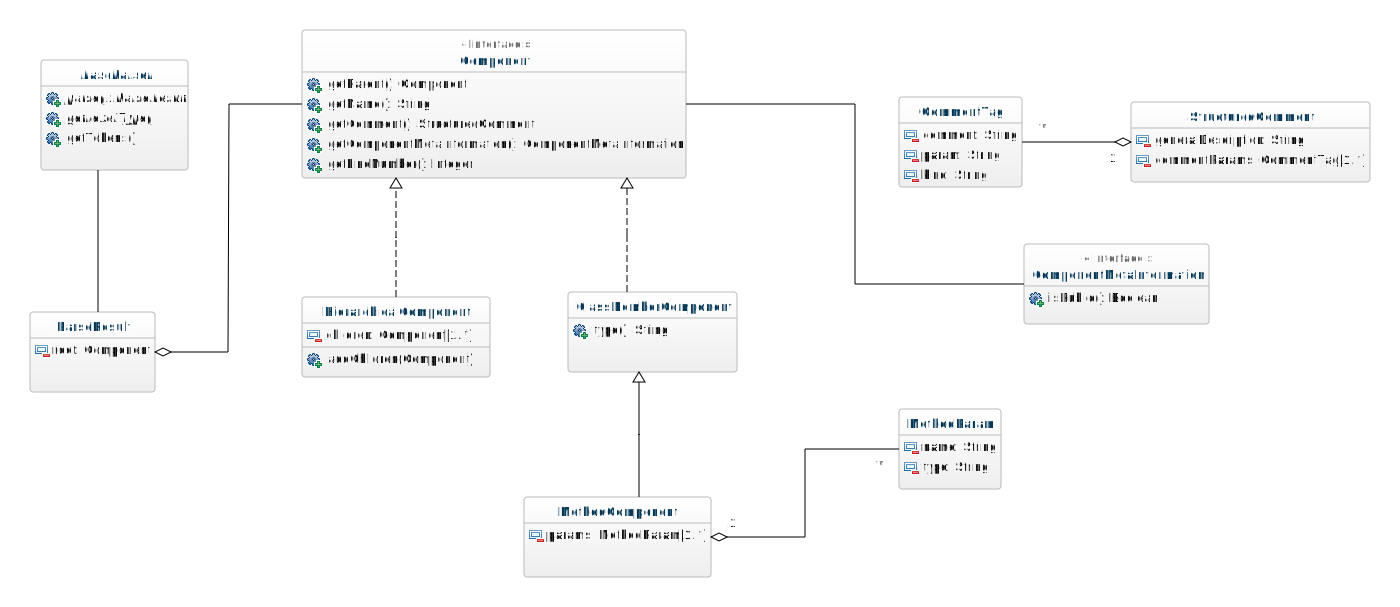
\includegraphics[height=9cm,keepaspectratio,angle=90]{figures/uml/parsing.png}
    \caption{UML-Diagramme aller Klassen, die relevant für das Parsen sind}
    \label{fig:uml_parsing}
\end{figure}
\chapter{UML-Diagramm: Metriken}
\begin{figure}[ht!]
\fontsize{5}{10}\selectfont
    \centering
    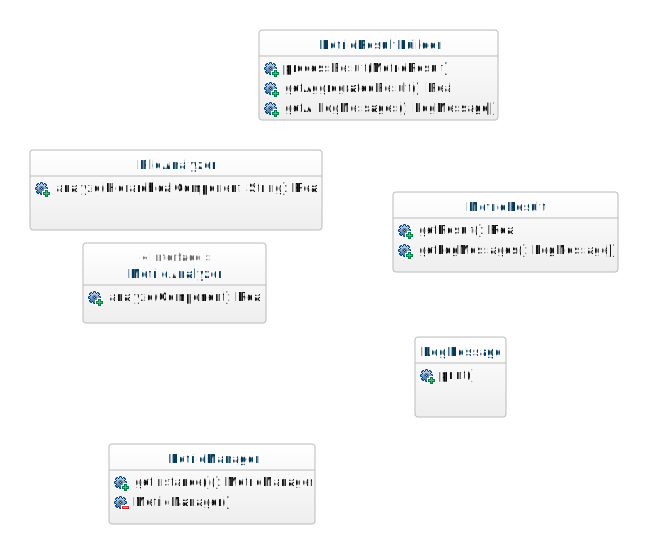
\includegraphics[height=10cm,keepaspectratio,angle=90]{figures/uml/metriken.png}
    \caption{UML-Diagramme aller Klassen, die relevant für die Metriken sind}
    \label{fig:uml_metrics}
\end{figure}
\chapter{Konfiguration des Tools}
\begin{description}
        \item[include]  Alle Dateien, die bei der Bewertung der Dokumentationsqualität berücksichtigt werden müssen
        \item[Exclude]  Teilmenge von include, enthält Dateien, die nicht weiter betrachtet werden müssen
        \item[metrics]  Alle Metriken, die das Tool verwenden soll. Dies ist ein Array von Objekten mit der Struktur \enquote{(name,weight,unique\_name,params)}, wobei \textit{weight} das Gewicht der jeweiligen Metrik ist( Bei Algorithmen ohne Relevanz des Gewichts wird es ignoriert), \textit{name} der Name (oder Aliasname) der Metrik und \textit{params} ein Objekt mit den Parametern der Metrik
        \item[absolute\_threshold] Mindestwert der Bewertung, die erreicht werden muss, sonst wird die Dokumentationsqualität nicht akzeptiert
       
          \item[builder] Der Algorithmus/\textit{ResultBuilder}, der die einzelnen Ergebnisse verarbeitet.
        
        \item[parser]  Kann verwendet, um die zu parsende Programmiersprache zu wählen. Dazu muss \textit{ParserFactory} angepasst werden
        
        \item[path\_weights] Ein Array von Objekten der Struktur \enquote{(path,weight)}. Wird verwendet, um einzelne Pfade höher oder niedriger zu gewichtet
        
         \item[component\_weights] Ein Array von Objekten der Struktur \enquote{(name,weight)}. Wird verwendet, um einzelne Komponenten höher oder niedriger zu gewichtet
         
         \item[default\_path\_weight] Das Standardgewicht für eine Datei, wenn keine passende Gewichtung gefunden wurde
         
         \item[default\_component\_weight] Das Standardgewicht einer Komponente, wenn keine passende Gewichtung gefunden wurde
         
         \item[state\_manager] Kann verwendet werden, um festzulegen, wie das letzte Ergebnis der Dokumentationsqualität gespeichert werden soll. Weitere Möglichkeiten können durch Erweiterung der \textit{StateManagerFactory} hinzugefügt werden.
         
         \item[relative\_threshold] Der maximale  relative Abstand zur letzten Dokumentationsqualität bevor eine Fehlermeldung geworfen wird.
        
        
        
    \label{enum:tool_javadoc_conf}
\end{description}
\chapter{Implementierte Metriken}\label{appendix_metrics}
\section{Anteil dokumentierter Komponenten an allen Komponenten}
\begin{description}
    \item [Metrikname]  simple\_comment
    \item [Klassenname] SimpleCommentPresentMetric
    \item[Beschreibung] Berechnet den Anteil der dokumentierten Komponenten an allen Komponenten, kann Getter und Setter ignorieren
\end{description}

\section{Anteil öffentlicher dokumentierter Komponenten an allen öffentlichen Komponenten}
\begin{description}
    \item [Metrikname]  public\_members\_only
    \item [Klassenname] SimplePublicMembersOnlyMetric
    \item[Beschreibung] Berechnet den Anteil der öffentlichen dokumentierten Komponenten an allen öffentlichen Komponenten, kann Getter und Setter ignorieren
\end{description}

\section{Bestrafung langer undokumentierter Methoden}
\begin{description}
    \item [Metrikname]  large\_method\_commented
    \item [Klassenname] SimpleLargeMethodCommentedMetric
    \item[Beschreibung] Bestraft undokumentierte Methoden je nach ihrer Länge
\end{description}

\section{Vollständigkeit der Dokumentation von Methoden}
\begin{description}
    \item [Metrikname]  method\_fully\_documented
    \item [Klassenname] SimpleMethodDocumentationMetric
    \item[Beschreibung] Prüft, ob alle Methodenparameter und Rückgabewert dokumentiert sind
\end{description}

\section{Anteil dokumentierter Methoden an allen Methoden unter
Berücksichtigung der LOC}
\begin{description}
    \item [Metrikname]  commented\_lines
    \item [Klassenname] CommentedLinesRatioMetric
    \item[Beschreibung]  Berechnet den Anteil der \ac{LOC} der dokumentierten Methoden an allen \ac{LOC} aller Methoden
\end{description}

\section{Kohärenz zwischen Kommentar und
Komponentenname}
\begin{description}
    \item [Metrikname]  comment\_name\_coherence
    \item [Klassenname] CommentNameCoherenceMetric
    \item[Beschreibung]  Prüft, ob der Kommentar und der Name der dokumentierten Komponente sehr ähnlich sind oder keine Ähnlichkeit haben, arbeitet nur mit Methoden
\end{description}

\section{Verwendung bestimmter Wörter bestrafen}
\begin{description}
    \item [Metrikname]  certain\_terms
    \item [Klassenname] CertainTermCountMetric
    \item[Beschreibung]  Bestraft das Vorkommen bestimmter Wörter (wie z.~B. Abkürzungen)
\end{description}

\section{Bewertung der Formatierung}
\begin{description}
    \item [Metrikname]  formatting\_good
    \item [Klassenname] FormattingGoodMetric
    \item[Beschreibung] Überprüft, ob korrekte Tags verwendet wurde, HTML-Tags geschlossen wurden und bei langen Methoden überhaupt eine Formatierung verwendet wurden
\end{description}


\section{Bewertung der Formatierung}
\begin{description}
    \item [Metrikname]  spellling
    \item [Klassenname] SpellingMetric
    \item[Beschreibung]Sucht nach Rechtschreibfehlern und bestraft sie
\end{description}

\section{Erwähnung von Randfällen bei Methodenparameter
und -rückgabewerte}
\begin{description}
    \item [Metrikname]  edge\_case
    \item [Klassenname] EdgeCaseMetric
    \item[Beschreibung] Prüft, ob bei der Dokumentation von Parametern die Behandlung des Wertes \textit{null} erwähnt wird
\end{description}


\section{Gunning-Fog-Index}
\begin{description}
    \item [Metrikname]  gunning\_fog
    \item [Klassenname] GunningFogMetric
    \item[Beschreibung] Berechnet den Gunnin-Fog-Index des Kommentars und bewertet so, ob der Kommentar verständlich ist
\end{description}
 

\begin{comment}
\begin{table}[ht!]
    \centering
    \begin{tabular}{m{4.5cm}|m{6.8cm}|m{5cm}}
        \textbf{Metrikname} & \textbf{Klassenname} & \textbf{Beschreibung}  \\\hline
          simple\_comment & SimpleCommentPresentMetric & Berechnet den Anteil der dokumentierten Komponenten an allen Komponenten\\\hline
        public\_members\_only & SimplePublicMembersOnlyMetric &   Berechnet den Anteil der öffentlichen dokumentierten Komponenten an allen öffentlichen Komponenten\\\hline
        large\_method\_commented & SimpleLargeMethodCommentedMetric & Bestraft undokumentierte Methoden je nach ihrer Länge\\\hline
     method\_fully\_documented & SimpleMethodDocumentationMetric & Prüft, ob alle Methodenparameter und Rückgabewert dokumentiert sind\\\hline
       commented\_lines\_ratio& CommentedLinesRatioMetric & Berechnet den Anteil der \ac{LOC} der dokumentierten Methoden an allen \ac{LOC} aller Methoden\\\hline
       flesch& FleschMetric & Berechnet den Flesch-Score des Kommentars und bewertet so, ob der Kommentar verständlich ist\\\hline
        comment\_name\_coherence&CommentNameCoherenceMetric & Prüft, ob der Kommentar und der Name der dokumentierten Komponente sehr ähnlich sind oder keine Ähnlichkeit haben\\\hline
     certain\_terms&CertainTermCountMetric & Bestraft das Vorkommen bestimmter Wörter (wie z.~B. Abkürzungen)\\\hline
          formatting\_good&FormattingGoodMetric & Überprüft, ob korrekte Tags verwendet wurde, HTML-Tags geschlossen wurden und bei langen Methoden überhaupt eine Formatierung verwendet wurden\\\hline
          spellling&SpellingMetric & Sucht nach Rechtschreibfehlern und bestraft sie\\\hline
        edge\_case&EdgeCaseMetric & Prüft, ob bei der Dokumentation von Parametern die Behandlung des Wertes \textit{null} erwähnt wird\\\hline
        gunning\_fog&GunningFogMetri& Berechnet den Gunnin-Fog-Index des Kommentars und bewertet so, ob der Kommentar verständlich ist\\
    \end{tabular}
    \caption{Alle implementierten Metriken}
    \label{table:metrics_name}
\end{table}
\end{comment}

\chapter{Rohdaten der Geschwindigkeitsmessung}\label{chapter:raw_speed_data}
\begin{table}[]
    \centering
    \begin{tabular}{c|c|c}
DE & CS &PMD\\\hline
2.633 &	2.483&	1.824\\\hline
		
2.640&	2.458&	1.807\\\hline
		
2.544&	2.315&	2.007\\\hline
		
2.533&	2.260&	1.971\\\hline
		
2.602&	2.285&	1.882\\\hline
		
2.404&	2.275&	2.024\\\hline
		
2.514&	2.645&	1.942\\\hline
		
2.412&	2.239&	1.917\\\hline
		
2.579&	2.744&	1.890\\\hline
		
2.522&	2.215&	1.897\\\hline
  \end{tabular}
    \caption{Benötigte Zeitdauer bei Log4J in Sekunden}
    \label{tab:raw_log4j}
\end{table}


\begin{table}[]
    \centering
    \sisetup{round-mode=places,round-precision=3}
    \begin{tabular}{c|c|c}
DE & CS &PMD\\\hline

16.719&	9.384&	8.036\\\hline
		
17.111&	9.431&	7.631\\\hline
		
16.715&	9.212&	7.658\\\hline
		
17.089&	9.414&	8.197\\\hline
		
16.486&	9.169&	7.985\\\hline
		
16.934&	9.303&	7.918\\\hline
		
17.003&	9.387&	7.884\\\hline
		
17.033&	9.269&	7.913\\\hline
		
16.997&	9.299&	7.916\\\hline
		
16.712&	9.268&	7.944\\\hline
    \end{tabular}
    \caption{Benötigte Zeitdauer bei ArgoUML in Sekunden}
    \label{tab:raw_argo}
\end{table}


\begin{table}[]
    \centering
    \begin{tabular}{c|c|c}
DE & CS &PMD\\\hline
69.867&27.581&22.235\\\hline
69.179&27.439&21.843\\\hline
69.118&27.849&21.738\\\hline
69.038&27.285&21.594\\\hline
68.620&27.079&21.561\\\hline
68.409&27.216&21.451\\\hline
69.765&27.346&21.178\\\hline
74.260&27.226&21.577\\\hline
70.197&27.239&21.558\\\hline
69.018&27.909&21.880\\\hline
    \end{tabular}
    \caption{Benötigte Zeitdauer bei Eclipse JDT in Sekunden}
    \label{tab:raw_eclipse}
\end{table}
\chapter{Boxplots: Geschwindigkeitsevaluation}\label{appendix:boxplots}
Nachfolgend werden die Boxplots aus Kapitel \ref{chapter:eval_speed_result} in vergrößerter Darstellung aufgeführt:
 \begin{figure}[ht!]
\includesvg[width=0.96\textwidth]{figures/chapter5/log4j_speed_boxplot.svg}
    \caption{Boxplot: Log4J}
  
\end{figure}
\hfill
 \begin{figure}
    \centering
\includesvg[width=\textwidth]{figures/chapter5/argo_speed_boxplot.svg}
    \caption{Boxplot: ArgoUML}
  
\end{figure}

 \begin{figure}
    \centering
\includesvg[,width=\textwidth]{figures/chapter5/eclipse_speed_boxplot.svg}
    \caption{Boxplot: Eclipse \ac{JDT} }
  
\end{figure}
\end{appendices}
	



\chapter*{Erklärung zur selbstständigen Abfassung der Masterarbeit}

Ich versichere, dass ich die eingereichte Masterarbeit selbstständig und ohne unerlaubte Hilfe verfasst habe. Anderer als der von mir angegebenen Hilfsmittel und Schriften habe ich mich nicht bedient. Alle wörtlich oder sinngemäß den Schriften anderer Autoren entnommenen Stellen habe ich kenntlich gemacht. \\


\bigskip
\bigskip
\bigskip
\bigskip
\noindent
Osnabrück, 18. Oktober 2018 \\

\bigskip
\bigskip
\bigskip
\bigskip
\noindent
Vorname Nachname
\end{document}

